% \section{Praktiken}

% \subsection{Fachpraxis}

\subsection{Application-Performance-Monitoring (APM)}

In der Fachpraxis haben sich über die Jahre einige Technologien entwickelt und etabliert, welche die Nachvollziehbarkeit von Anwendungsverhalten und Nutzerinteraktion ermöglichen oder verbessern. Auf Basis der zuvor vorgestellten Methoden und teils neuer Ansätze haben sich in der Wirtschaft einige Praktiken entwickelt. Eines dieser Ansätze ist das Application-Performance-Monitoring (APM, teils auch Application-Performance-Management).

APM lässt sich nicht simpel definieren, denn es existiert kein Konsens, welche Eigenschaften und Funktionalitäten ein APM umfasst. Ahmed \etal \cite{StudyingTheEffectivenessOfAPMTools}, Heger \etal \cite{APMStateOfTheArtAndChallenges}, Rabl \etal \cite{SolvingBigDataChallengesForAPM} sowie Dynatrace \cite{DynatraceAPM} definieren, dass APM eine Menge an Methoden, Techniken und Werkzeugen umfasst, die das System konstant überwachen und Aufschluss über den Zustand geben, sodass die Verfügbarkeit des Systems sichergestellt werden kann. Anders definieren dies jedoch Santos Filipe \cite{ClientSideMonitoringOfDistributedSystems}, New Relic \cite{NewRelicAPM} und Gartner \cite{GartnerMagicQuadrantForAPM}, welche APM weniger allgemeingültig definieren, sondern APM eher über explizite Teilaspekte definieren, die es erfüllen muss, damit es sich um ein konformes APM handelt. Jedoch existiert hier ebenso kein Konsens, welche expliziten Aspekte erfüllt sein müssen, damit ein Monitoring-System zu einem APM wird.

In dieser Arbeit wird auf Basis der ersten und eher allgemeingültigen Definition ein APM so definiert: APM befasst sich mit dem Beobachten eines Softwaresystems und der Gewinnung von relevanten Daten aus diesem System zur näheren Analyse, um zu ermöglichen, dass Rückschlüsse über die Gesundheit des Systems gezogen werden können und so die Verfügbarkeit sichergestellt werden kann. Um dies zu erreichen, lassen sich grob 5 Fachgebiete differenzieren, die unterschiedliche Aspekte eines Softwaresystems aufdecken \cite{ASurveyOfCloudMonitoringTools} \cite{GartnerMagicQuadrantForAPM} \cite{ResearchAndApplicationOfOperatingMonitoring}:

\begin{enumerate}
	\item Infrastruktur-Monitoring (IM)
	\item Application-and-Service-Monitoring (ASM)
	\item Real-User-Monitoring (RUM)
	\item Error-Monitoring
	\item Distributed-Tracing
\end{enumerate}

\subsubsection{Infrastructure-Monitoring (IM)}

Infrastructure-Monitoring beschäftigt sich hauptsächlich mit der Überwachung der Infrastruktur. Hierbei wird bspw. die Verfügbarkeit von Netzwerkressourcen überwacht sowie die Auslastung von Hard- und Softwareressourcen. Dieses Monitoring kann ohne Anpassungen der Software erfolgen und stellt somit ein Beispiel für Black-Box-Monitoring dar \cite{ClientSideMonitoringOfDistributedSystems}. Beispielsweise ist die Überwachung von CPU- und Speicherausnutzung eines Containers Teil von Infrastructure-Monitoring.

\subsubsection{Application-and-Service-Monitoring (ASM)}

Anders als beim System-Monitoring handelt es sich bei Application-and-Service-Monitoring (ASM, teilweise auch Application-Component-Monitoring) um White-Box-Monitoring. Genauer bedeutet dies, dass die Softwarekomponenten angepasst werden müssen, sodass innerhalb der Laufzeitumgebungen Daten gesammelt werden können. Beispielsweise werden die Antwortzeit von Schnittstellaufrufen protokolliert und systematisch überwacht. Auf Basis der Daten lassen sich u. A. Abweichungen von der Norm feststellen, von einzelnen Systemen oder vom aktuellen Gesamtsystem zu einem vorherigen Zeitpunkt.

\subsubsection{Real-User-Monitoring (RUM)}

\nomenclature[Fachbegriff]{UI}{User-Interface}

Real-User-Monitoring beschäftigt sich mit dem Mitschneiden von allen Nutzerinteraktionen und Umgebungseigenschaften einer Benutzeroberfläche \cite{IdentifyingWebPerformanceDegradations}. Um diese Daten zu ermitteln ist eine Änderung der Software für die Benutzeroberfläche notwendig, welches RUM zu einem White-Box-Monitoring macht. RUM wird jedoch nicht dazu verwendet, die Interaktionen eines einzelnen Nutzers aufzudecken, sondern Aufschluss über die gesamte Nutzerschaft der Anwendung zu erhalten. Die Daten werden oftmals gruppiert bspw. nach den Interaktionen oder auch nach Umgebungseigenschaften, wie dem Browser der Nutzer. Durch die Gruppierung lassen sich Probleme der User-Experience feststellen \cite{AConceptLatticeForRecognitionOfUserProblems}, aber auch Leistungsprobleme der Anwendung feststellen und ob diese den unterschiedlichen Umgebungen der Nutzer geschuldet sind \cite{IdentifyingWebPerformanceDegradations}.

\subsubsection{Error-Monitoring}

Das Error-Monitoring konzentriert sich auf das Erfassen und Melden von Fehlern \cite{CrashbinCrashMonitoring}. Error-Monitoring lässt sich sowohl als White-Box- sowie als Black-Box-Monitoring umsetzen, da über existierende Protokollierung bereits Fehler festgestellt werden können, jedoch kann es hierbei sinnvoll sein eine Software anzupassen, um mehr Kontextinformationen zu erfassen. Das Error-Monitoring wird oftmals eng mit einem Issue-Management verbunden, um aufgetretene Fehler und deren Behebung nachzuhalten zu machen \cite{CrashbinCrashMonitoring}.

\subsubsection{Distributed-Tracing}

Beim Distributed-Tracing handelt es sich um die fortgeschrittene Art des Tracings, welche systemübergreifend den Durchlauf von Abfragen protokolliert (vgl. \autoref{sec:tracing}). Diese Art von Monitoring gibt, anders als die anderen Arten, keine Einsicht in einzelne Komponenten, sondern veranschaulicht die resultierenden Interaktionen einer Abfrage.

\subsection{Log-Management}

Neben dem APM gibt es zudem weitere Funktionalitäten, die Technologien in der Fachpraxis vorweisen, wie z. B. das Log-Management. Log-Management umfasst die Erfassung, Speicherung, Verarbeitung und Analyse von Logdaten von Anwendungen. Neben diesen Funktionen bieten solche Werkzeuge oftmals fundierte Suchfunktionen und Visualisierungsmöglichkeiten \cite{DesignLogManagementSystem}. Um die Daten aus einer Anwendung heraus zu exportieren, gibt es meist eine Vielzahl an Integrationen für Frameworks und Logbibliotheken.

Einer der wichtigsten Aspekte des Log-Managements, ist der Fähigkeit mit großen Datenmengen umzugehen und dabei den Nutzern zu ermöglichen auf diesen Daten zu arbeiten, Analysen durchzuführen und auch alte Datensätze abrufen zu können\cite{LoggingAndLogManagement}. Damit die teils enormen Datenmengen den Nutzer zur Verfügung stehen, aber gleichzeitig nicht das System beeinträchtigen, sind spezielle Architekturkonzepte erforderlich. Beispielsweise werden selten abgerufene oder alte Daten in einen Langzeitspeicher überführt, welcher für die Speicherung optimiert ist, aber im Gegenzug keine zeitlich effizienten Ergebnisse liefern kann \cite{LoggingAndLogManagement}.

\subsection{Session-Replay}

Session-Replay beschreibt das Vorgehen, eine Sitzung eines Nutzers nachzustellen, so als ob sie gerade passiert \cite{NoBoundariesExfiltrationBySessionReplayScripts}. Hierbei können einzelne Aspekte der Anwendung nachgestellt werden, bspw. der Kommunikationsablauf oder die DOM-Manipulationen. Je mehr Aspekte nachgestellt werden, desto realitätsnaher ist die Nachstellung und entsprechend hilfreich ist sie beim Nachvollziehen. Realitätsnahes Session-Replay nimmt somit eine enorme Datenmenge für jede Nutzersitzung auf und benötigt besonders bei Browsern eine effiziente Kommunikation, um die User-Experience (UX) nicht negativ zu beeinflussen \cite{AdvancedWebAnalyticsToolForMouseTracking} \cite{LogRocketPerformance}.

\begin{wrapfigure}[17]{r}{0.40\textwidth}
\centering
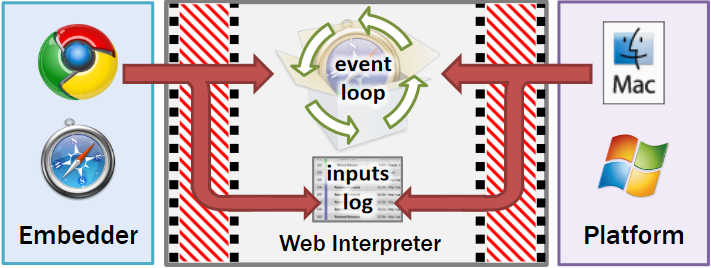
\includegraphics[width=\linewidth]{img/03_methoden/timelapse_figure5.png}
\caption{Mitschneiden von DOM-Events, Abb. aus \cite{TimelapsePaper}}
\label{fig:timelapse_figure5}
\smallskip\par
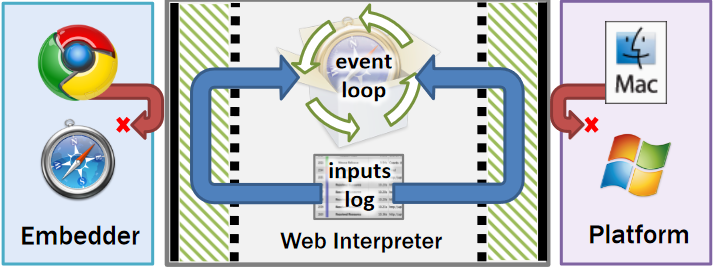
\includegraphics[width=\linewidth]{img/03_methoden/timelapse_figure6.png}
\caption{Abspielen von DOM-Events, Abb. aus \cite{TimelapsePaper}}
\label{fig:timelapse_figure6}
\end{wrapfigure}

Bereits 2013 entwickelten Burg \etal \cite{TimelapsePaper} mit \enquote{Timelapse} ein Framework, um Benutzersitzungen bei Webanwendungen aufzunehmen und wiederzugeben. Timelapse unterscheidet sich zu gängigen Session-Replay-Ansätzen dahingehend, dass die Wiedergabe keine vereinfachte Nachstellung der Anwendung ist. Stattdessen wird die JavaScript-Eventloop abgekapselt und es werden die Aufrufe von und zu der Eventloop mitgeschnitten (vgl. \autoref{fig:timelapse_figure5}).

Beim Abspielen werden die Aufrufe dann in derselben Reihenfolge an die Eventloop übergeben (vgl. \autoref{fig:timelapse_figure6}). Dies bedeutet es ist ein exaktes wiederholtes Ausführen in derselben Umgebung möglich und dies ermöglicht eine detaillierte Nachvollziehbarkeit des Anwendungsverhaltens. Leider wird für diesen Ansatz eine gepatchte Version von WebKit vorausgesetzt, somit wird auch Zugriff auf das Endnutzersystem benötigt. Aus diesem Grund und weil es sehr mehr als 5 Jahren nicht mehr gepflegt wird\footnote{Timelapse GitHub Repo \url{https://github.com/burg/replay-staging/}}, ist es ungeeignet für die hier angestrebte Lösung. Die vorgestellten Konzepte stellen jedoch nützliche Kernprinzipien für das Session Replay im Allgemeinen dar.